\documentclass[12pt]{article}
\usepackage[letterpaper, margin=1in]{geometry}
\usepackage{times}
\usepackage{helvet}
\usepackage{courier}
\usepackage{color}
\usepackage{multicol}
\usepackage{lipsum}
\usepackage{listings}
\usepackage{graphicx}
\usepackage{fancyhdr}
\usepackage{enumitem}
\usepackage[%  
    colorlinks=true,
    pdfborder={0 0 0},
    linkcolor=blue
]{hyperref}
\usepackage[all]{hypcap}
\usepackage{float}
\usepackage{textcomp}
\usepackage{placeins}
\usepackage[%
  autocite    = superscript,
  backend     = bibtex,
  sortcites   = true,
  style       = numeric,
]{biblatex}
\addbibresource{proposal.bib}

\setlist{noitemsep, topsep=0pt}

\begin{document}

{\Huge \textbf{FPGAirPods} Project Proposal}

\vspace{2mm}
{Gokul Kolady, Ben Kettle, Niko Ramirez | \today \ | 6.111}
\vspace{5mm}

\begin{multicols}{2}
\section{Overview}
Our 6.111 final project aims to implement active noise cancellation as seen in over- and in-ear headphones such as the Bose QC35 and the AirPods Pro (hence the name). In order to do this, we will first need to create a physical model of a single headphone (one ear cup) that we will use to test. Inside the ear cup, we will install a speaker (far from the ear) and a digital microphone (closer to the ear). We will also use a digital microphone external to the ear cup in order to capture ambient noise.

The FPGA itself will handle the computational side of the active noise cancellation. This will primarily involve an adaptive filter that will continually improve its coefficients in order to minimize the error function--ie, the noise that makes it through and is not cancelled out. We run the input from the external microphone through this filter, and play the filtered result out of the speaker with the aim of cancelling noise.

\section{Materials}
Several materials will be used in order to construct a prototype "headphone" to test on: 
\begin{itemize}
    \item 2x \href{https://www.adafruit.com/product/3421}{SPH0645LM4H microphone breakout boards} from Adafruit will be used to collect noise from inside and outside the ear cup. These communicate via I2S, which will remove the need for ADCs between the microphone and the FPGA, and minimize potential for noise in the wires from the FPGA to the earpiece.
    \item \href{https://www.adafruit.com/product/3968}{Speaker}
    \item \href{https://www.adafruit.com/product/3006}{Amplifier}? We could put this inside the cup, or we might be able to use the onboard amplifier on the FPGA--I'm not sure.
    \item Cup
    \item Foam
    \item Wire
\end{itemize}
\end{multicols}


\section{Block Diagram}

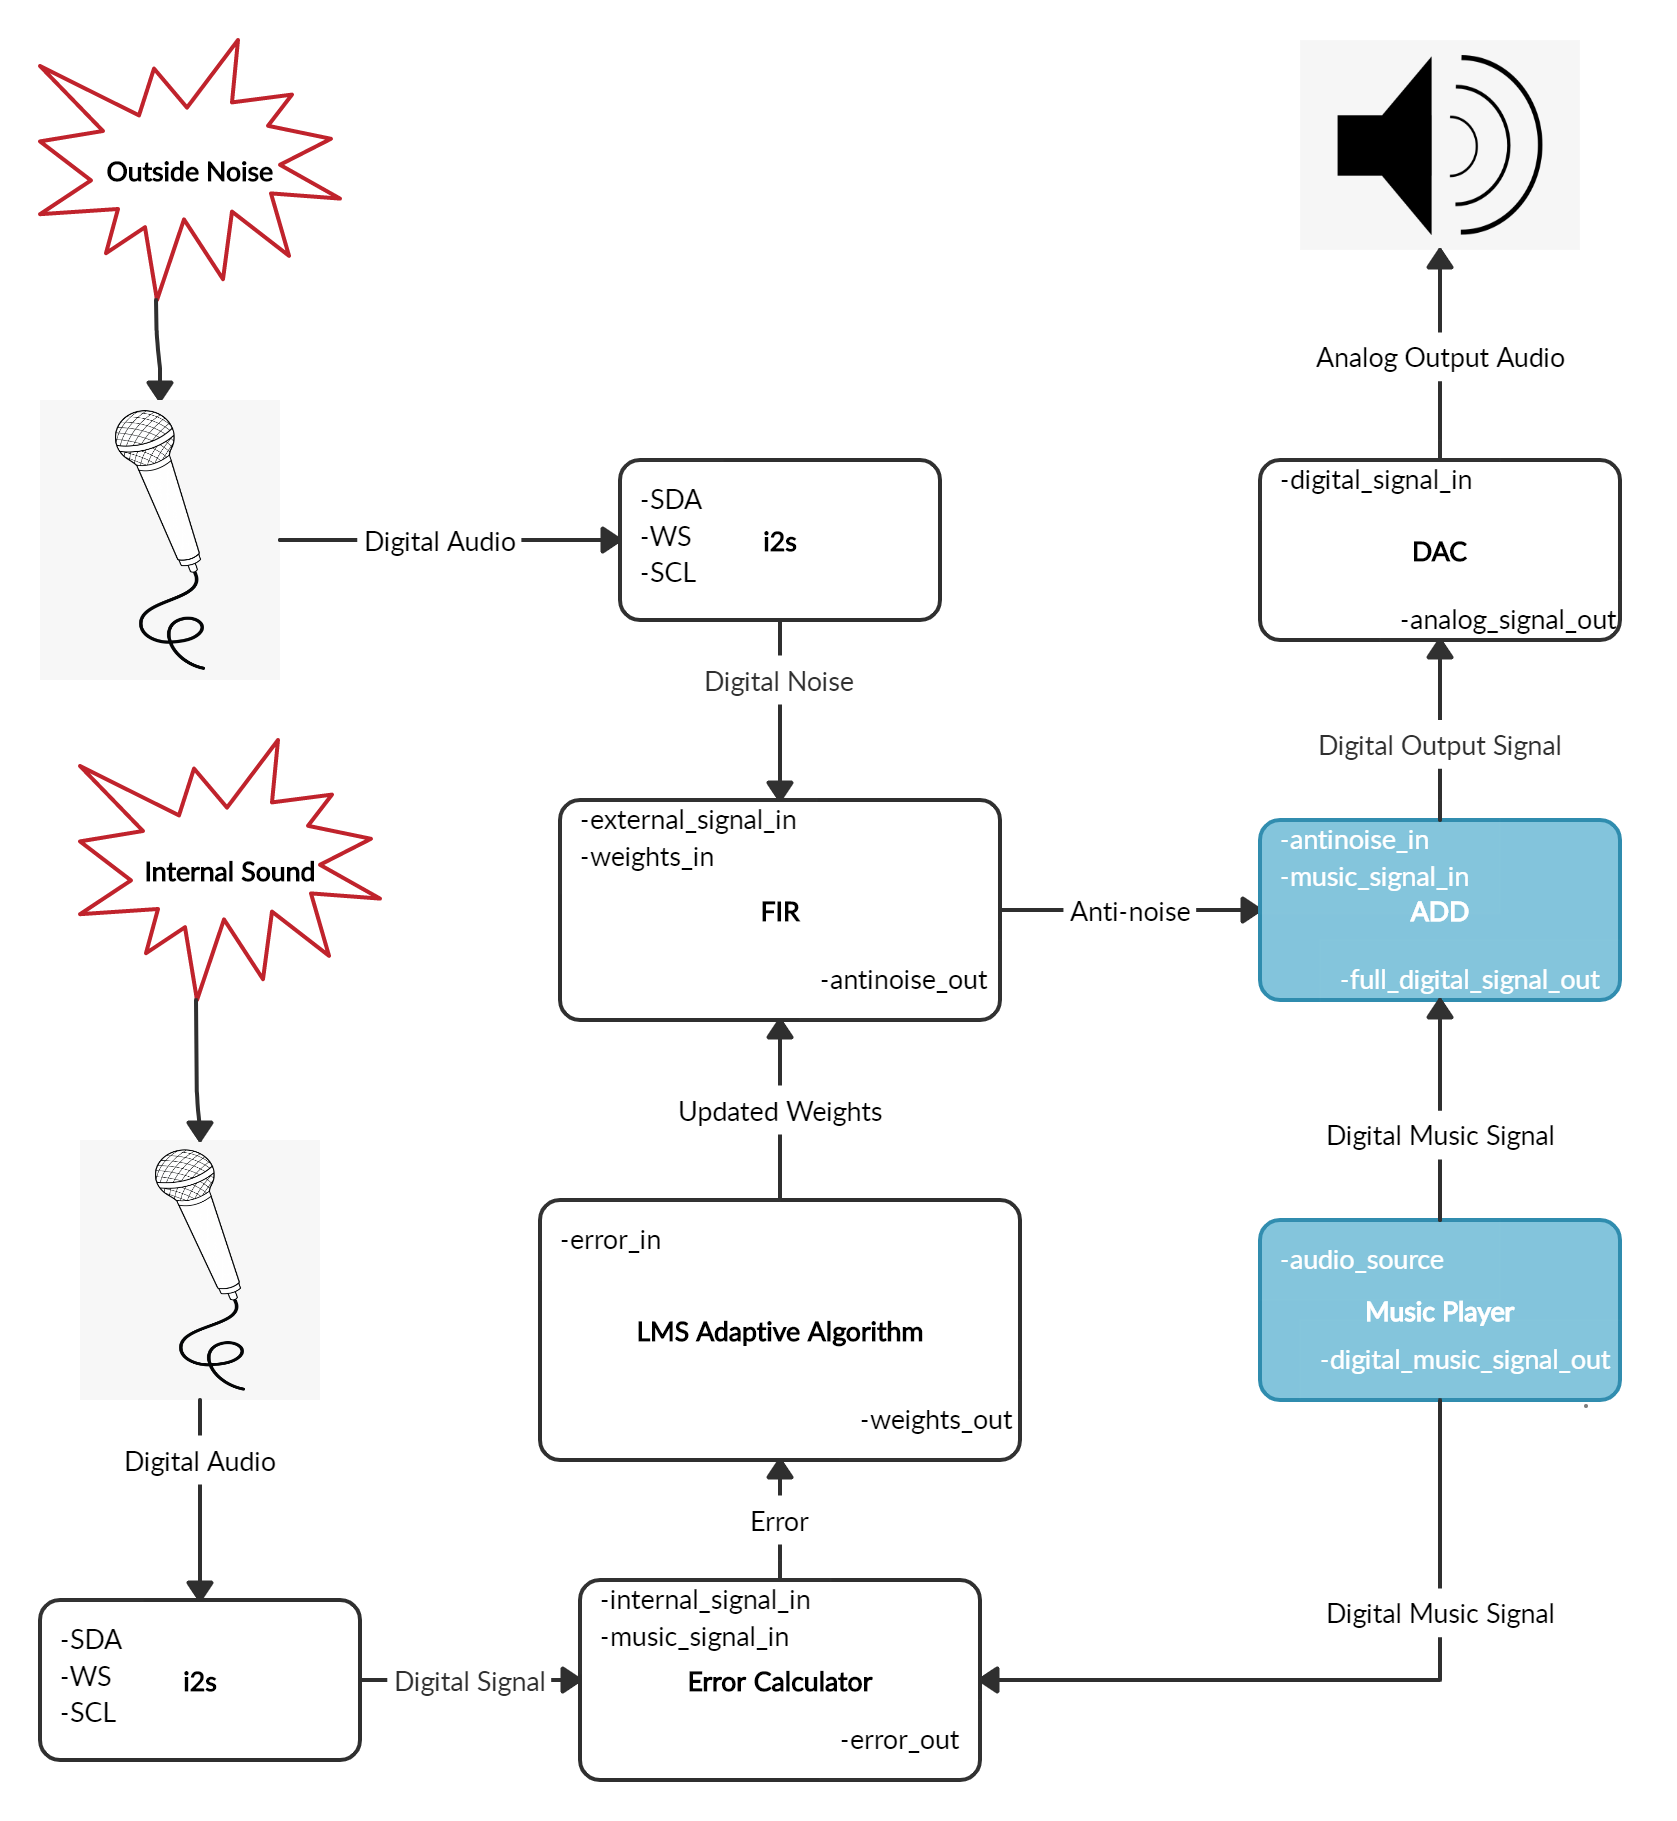
\includegraphics[width=\textwidth]{docs/proposal/images/Proposal Block Diagram.png}


\newpage
\section{Modules}
\begin{multicols}{2}
\subsection{I2S - \textit{IP}}
This module will parse the incoming data stream from each of the two microphones. Can be implemented with IP.
\subsubsection{Inputs}
\begin{itemize}
    \item SDA - Microphone Data
    \item SCL - Audio Clock
\end{itemize}
\subsubsection{Outputs}
\subsubsection{Level of Performance}
\begin{itemize}
    \item 476 LUTs
    \item 1722 FFs
    \item 1 36k BRAM
\end{itemize}

\subsection{FIR Filter - \textit{Owners}}
The FIR Filter module convolves the external ambient noise with a set of filter coefficients in order to produce an anti-noise signal. This anti-noise signal is later used to cancel out the ambient noise that makes it into the the ear cup. These coefficients are set continuously by the LMS adaptive algorithm module.
\subsubsection{Inputs}
blah
\subsubsection{Outputs}
blah
\subsubsection{Complexity}
blah
\subsubsection{Level of Performance}
blah
\subsubsection{Testing}
blah

\subsection{LMS Adaptive Algorithm}
This module uses the LMS adaptive algorithm in order to update the coefficients of the FIR Filter for better noise cancellation. This algorithm takes advantage of the steepest descent optimization method, which analyzes the impact of the previous filter coefficients on the observed error and computes appropriate adjustments. This update is accomplished using the following equation:

$$b_k(n + 1) = b_k(n) + \Lambda e(n)f(n-k)$$
$$k = 0, 1, 2,... M-1$$

VARIABLE DESCRIPTIONS
\subsubsection{Inputs}
blah
\subsubsection{Outputs}
blah
\subsubsection{Complexity}
blah
\subsubsection{Level of Performance}
blah
\subsubsection{Testing}
blah

\subsection{Error Calculator - \textit{Owners}}
The error calculator computes the difference between the output of the internal microphone (the sound within the ear cup) and the intended final audio. If we reach our stretch goal, the intended audio will be the music being inputted into the system. Otherwise, the goal will be silence. This difference or "error" will be fed into the LMS modules for error correction.
\subsubsection{Inputs}
blah
\subsubsection{Outputs}
blah
\subsubsection{Complexity}
blah
\subsubsection{Level of Performance}
blah
\subsubsection{Testing}
blah

\subsection{DAC - \textit{Owners}}
The DAC (Digital-to-Analog Converter) module will be used to transform the final digital output audio into an analog signal that can be played through the speaker.
\subsubsection{Inputs}
blah
\subsubsection{Outputs}
blah
\subsubsection{Complexity}
blah
\subsubsection{Level of Performance}
blah
\subsubsection{Testing}

\subsection{Music Player - \textit{Owners}}
This module outputs the source music/audio in digital form (the user should ideally hear a version of this audio with minimal corruption). With the possible extension of Bluetooth-based input audio, this module would be modified to receive its input from a Bluetooth receiver that would be interfaced with the FPGA.
\subsubsection{Inputs}
blah
\subsubsection{Outputs}
blah
\subsubsection{Complexity}
blah
\subsubsection{Level of Performance}
blah
\subsubsection{Testing}
blah

\subsection{Add - \textit{Owners}}
If we reach our stretch goal of the music player integration, we will need a module to merge the output of the FIR---the signal that will cancel the incoming noise---with the music to play. This module will take two signals as an input, and output their sum. It will be very simple.

\end{multicols}
Each module
\\-inputs and outputs
\\-complexity
\\-level of performance
\\(eg. number and type of arithmetic operations, size of internal memories, required throughput)
\\-how it will be tested

Teamwork Distribution
\\-team member works on which module 
\\-most modules should have a single designer
\\-testbenches should be different members

\printbibliography
\end{document}
